\chapter{Rate of SLSNe at z$\sim$1}
\label{Chapter3}
\lhead{Chapter 3. \emph{Rate of SLSNe}}

In this chapter I present the measurement of a volumetric rate of SLSNe at z$\sim$1 measured using the archival SNLS data. First I propose a photometric definition of a SLSN based on the modeling of light curves using the spin-down of a magnetar model followed by a search for missed objects within the SNLS dataset. I briefly introduce the new photometric sample before describing the Monte-Carlo simulation of the survey, aimed at measuring the rate and its uncertainties. Finally, I compare the value measured to those found in the literature and discuss the significance of the result in terms of the physical origin of the objects as well as their detectability by DES and other, future, surveys. The work presented in this chapter has been published in \citet{Prajs2016}.

\section{Defining a SLSN}
\label{sec:SLSNDefinition}
Our first task in the process of measuring the rate of SLSNe was to develop a method for the photometric selection of optical transients that were to enter our SLSN sample. The earliest definitions of SLSNe relied on their peak luminosity and often defined them as SN with an absolute $u$-band magnitude of $M_{u}<-21$ \citep{2012Sci...337..927G}. It was our view that this definition is not adequate for our search for two main reasons. The first was that, already at that time, there existed several examples in the literature of events that are spectroscopically similar to SLSNe, but that do not pass this arbitrary threshold. Some of these events included DES13S2cmm \citep{2015MNRAS.449.1215P} and PTF11rks \citep{2013ApJ...770..128I} which both had M$_u$ > -21 but are also associated with a very slow evolution which is synonymous with SLSNe. The second reasons was the discovery of new classes of fast and luminous transients \citep{2016ApJ...819...35A} with luminosities similar to SLSNe, but with a faster light curve evolution and different spectroscopic types. Therefore, instead of an arbitrary luminosity cut, we use a photometric classification approach based on modeling SLSNe using the spin-down of a magnetar model as a simple analytical model that provides a good fit to a sample of confirmed SLSNe.

This approach did, however, have its drawbacks. Use of an analytical model implied that the rate was calculated only for objects which are similar to the sample of confirmed SLSNe, as presented in \sref{sec:litSample}. We were aware that this would likely not capture all objects of this class at the time this work was undertaken but without a better definition of a SLSN more significant progress could not be achieved. In \cref{Chapter5} I present a more significantly more complex approach to this problem, as applied to DES, based on an artificial training sample of SLSNe and Machine Learning classifiers.

\subsection{Modeling SLSNe}
In order to model SLSN we required two main ingredients: an underlying model for the time-dependent bolometric luminosity of a SLSN, and an SED that can convert this bolometric luminosity into time-evolving spectra. This together forms a spectral series from which we can synthesis the photometry in any desired filter and at any desired redshift. This can then be used for comparison to observed data. For the purpose of this chapter the exact form or the physical meaning behind the light curve model parameters are irrelevant as, in theory, any model that satisfactorily replicates the observables could be used for this purpose. I therefore provide only a brief overview of the model here while the remaining details are described in \sref{sec:SLAP}.

\subsubsection{Magnetar model}
The spin-down of a magnetar model assumes that a collapse of a giant star with an initial mass of M $>$ 40M$_{\odot}$ produces a SNIc like explosion whilst giving birth to a magnetar; a highly magnetized neutron star with a rotation period on the time scale of milliseconds \citep{Kasen2009,Woosley2010,Inserra2013}. The simple toy model assumes a spherically symmetric ejecta and a constant opacity. The free parameters in the model are the Magnetic field, $B_{14}$, spin period, $P_{\mathrm{ms}}$ and the diffusion timescale $\tau_M$ which is directly proportional to the ejecta mass, M$_{\mathrm{ej}}$ and the time of explosion, $t_{\mathrm{expl}}$.

\subsubsection{Fitting literature light curves}
The magnetar model provideded a good fit to all the SLSNe that formed part of our training sample. \tref{table:Magnetar} contains the model's best-fit parameters, as well as two additional derived observables which help us to identify the nature of the events without visually inspecting the light curves. These were the peak absolute magnitude in the SDSS $u$-band filter as well as the rise-time, $t_\mathrm{rise}$, of the SN as measured from explosion to maximum light in the rest-frame $u$-band. It is important to note here that the absolute magnitude, $M_u$, are given in the AB magnitude system. The zero-point correction factor betwee the AB and Vega magnitude system for the $u$-band filter is: $M_u^{\mathrm{AB}}\simeq M_u^{\mathrm{vega}}+0.9$ \citep{2007AJ....133..734B}. Therefore, while some of the training sample have $M_u^{\mathrm{AB}}>-21$, none have $M_u^{\mathrm{vega}}>-21$ which agrees with the previous definition of a SLSN.

\begin{table}
\begin{center}
\caption{Magnetar model parameters for the sample of 15 published SLSNe.}
\label{table:Magnetar}
\begin{tabular}{|l|r|r|r|r|r|r|r|r|r|r|}
\hline
  \multicolumn{1}{|c|}{Name} &
  \multicolumn{1}{c|}{$M_u$} &
  \multicolumn{1}{c|}{$t_\mathrm{rise}$} &
  \multicolumn{1}{c|}{$\tau_\mathrm{m}$} &
  \multicolumn{1}{c|}{$B_{14}$} &
  \multicolumn{1}{c|}{$P_{\mathrm{ms}}$} &
  \multicolumn{1}{c|}{$t_\mathrm{expl}$} &
  \multicolumn{1}{c|}{$E(B-V)$} &
  \multicolumn{1}{c|}{$\chi^2_{\nu}$} &
  \multicolumn{1}{c|}{Template} \\ & &
  \multicolumn{1}{c|}{(days)} &
  \multicolumn{1}{c|}{(days)} &
  \multicolumn{1}{c|}{($\times10^{14}$ G)} &
  \multicolumn{1}{c|}{(ms)} &
  \multicolumn{1}{c|}{(MJD)} & \\
\hline
  PTF12dam & -21.4 & 34.72 & 22.15 & 0.78 & 2.85 & 56044.5 & 0.18 & 2.49 & 06D4eu\\
  SN2011ke & -21.2 & 24.84 & 30.61 & 3.67 & 2.13 & 55647.5 & 0.01 & 1.31 & iPTF13ajg\\
  SN2010gx & -21.7 & 24.56 & 30.36 & 3.20 & 1.54 & 55247.1 & 0.19 & 0.86 & 06D4eu\\
  SN2013dg & -21.2 & 25.37 & 28.05 & 3.30 & 2.75 & 56412.3 & 0.07 & 0.23 & SCP06F6\\
  PS1-11ap & -21.8 & 32.1 & 20.08 & 0.79 & 2.51 & 55559.0 & 0.02 & 1.62 & 06D4eu\\
  DES14X3taz & -21.7 & 47.21 & 26.16 & 0.23 & 1.67 & 57019.2 & 0.09 & 5.18 & 06D4eu\\
  PS1-10bzj & -21.2 & 22.17 & 18.44 & 2.65 & 3.84 & 55524.0 & 0.07 & 0.37 & 06D4eu\\
  DES13S2cmm & -20.0 & 30.7 & 21.19 & 1.28 & 5.29 & 56509.0 & 0.01 & 0.51 & 06D4eu\\
  iPTF13ajg & -22.4 & 31.45 & 33.41 & 1.57 & 1.32 & 56346.9 & 0.19 & 0.30 & iPTF13ajg\\
  07D2bv & -21.1 & 28.41 & 36.88 & 3.40 & 2.18 & 54132.4 & 0.05 & 0.41 & SCP06F6\\
  06D4eu & -21.9 & 21.48 & 29.94 & 3.82 & 1.00 & 53956.3 & 0.11 & 1.26 & 06D4eu\\
\hline\end{tabular}
\end{center}
\end{table}

\subsubsection{Defing a SLSN parameter space}
\fref{fig:SLAPparam} shows the best-fit magnetar model parameter space. In order to define a region of the parameter space that defines a SLSN we inclosed the cluster of our literature points with an ellipsoid. We chose the lowest volume, simplest geometric body that was consistent with all the SLSN in our training sample. The ellipsoid was defined in terms of the three main fit parameters of the magnetar model, $\tau_\mathrm{m}$, $B_{14}$ and $P_{\mathrm{ms}}$. In the Cartesian coordinate system a position on any generic ellipsoid can be defined using \eref{eq:Ellipsoid}.

\begin{equation}
\label{eq:Ellipsoid}
\left( \begin{matrix}
x \\
y \\
z
\end{matrix} \right)
=
\mathbf{A}
\left( \begin{matrix}
R_x\cos(u)\cos(v) \\
R_y\cos(u)\sin(v) \\
R_z\cos(v)
\end{matrix} \right)
+ \mathbf{C}
\end{equation}

\noindent where \textbf{A} is a rotation matrix, \textbf{R} is the radius of the ellipsoid and \textbf{C} is the position of its center. The following conditions must be satisfied: $-\pi /2 \leq u \leq \pi /2$ and $-\pi \leq v \leq \pi$. We have set up our parameter space such that $\tau_\mathrm{m}$ lays along the $x$-axis, $B_{14}$ is along the $y$-axis and $P_{\mathrm{ms}}$ corresponding to the $z$-axis. Using the Khachiyan Algorithm \citep{Aspvall19801,KHACHIYAN198053}, we have performed an analytical fit to determine the ellipsoid that best describes the known population of SLSNe. We found the ellipsoid to have the following properties:

\begin{equation}
\label{eq:A}
\mathbf{A} =
\left( \begin{matrix}
-0.184 & 0.575 & -0.797\\
 0.008 & 0.812 & 0.586\\
0.983 & 0.102 & -0.154
\end{matrix} \right)
\end{equation}

\begin{equation}
\label{eq:R}
\mathbf{R} =
\left( \begin{matrix}
R_x \\
R_y \\
R_z
\end{matrix} \right)
=
\left( \begin{matrix}
1.89\\
2.17\\
11.32
\end{matrix} \right)
\end{equation}

\begin{equation}
\label{eq:C}
\mathbf{C} =
\left( \begin{matrix}
26.76 \\
2.14\\
2.77
\end{matrix} \right)
\end{equation}

\noindent \fref{fig:SLAPparam} shows the three, two-dimensional projections of this parameter space, populated with our training sample of literature SLSNe.

\begin{figure}
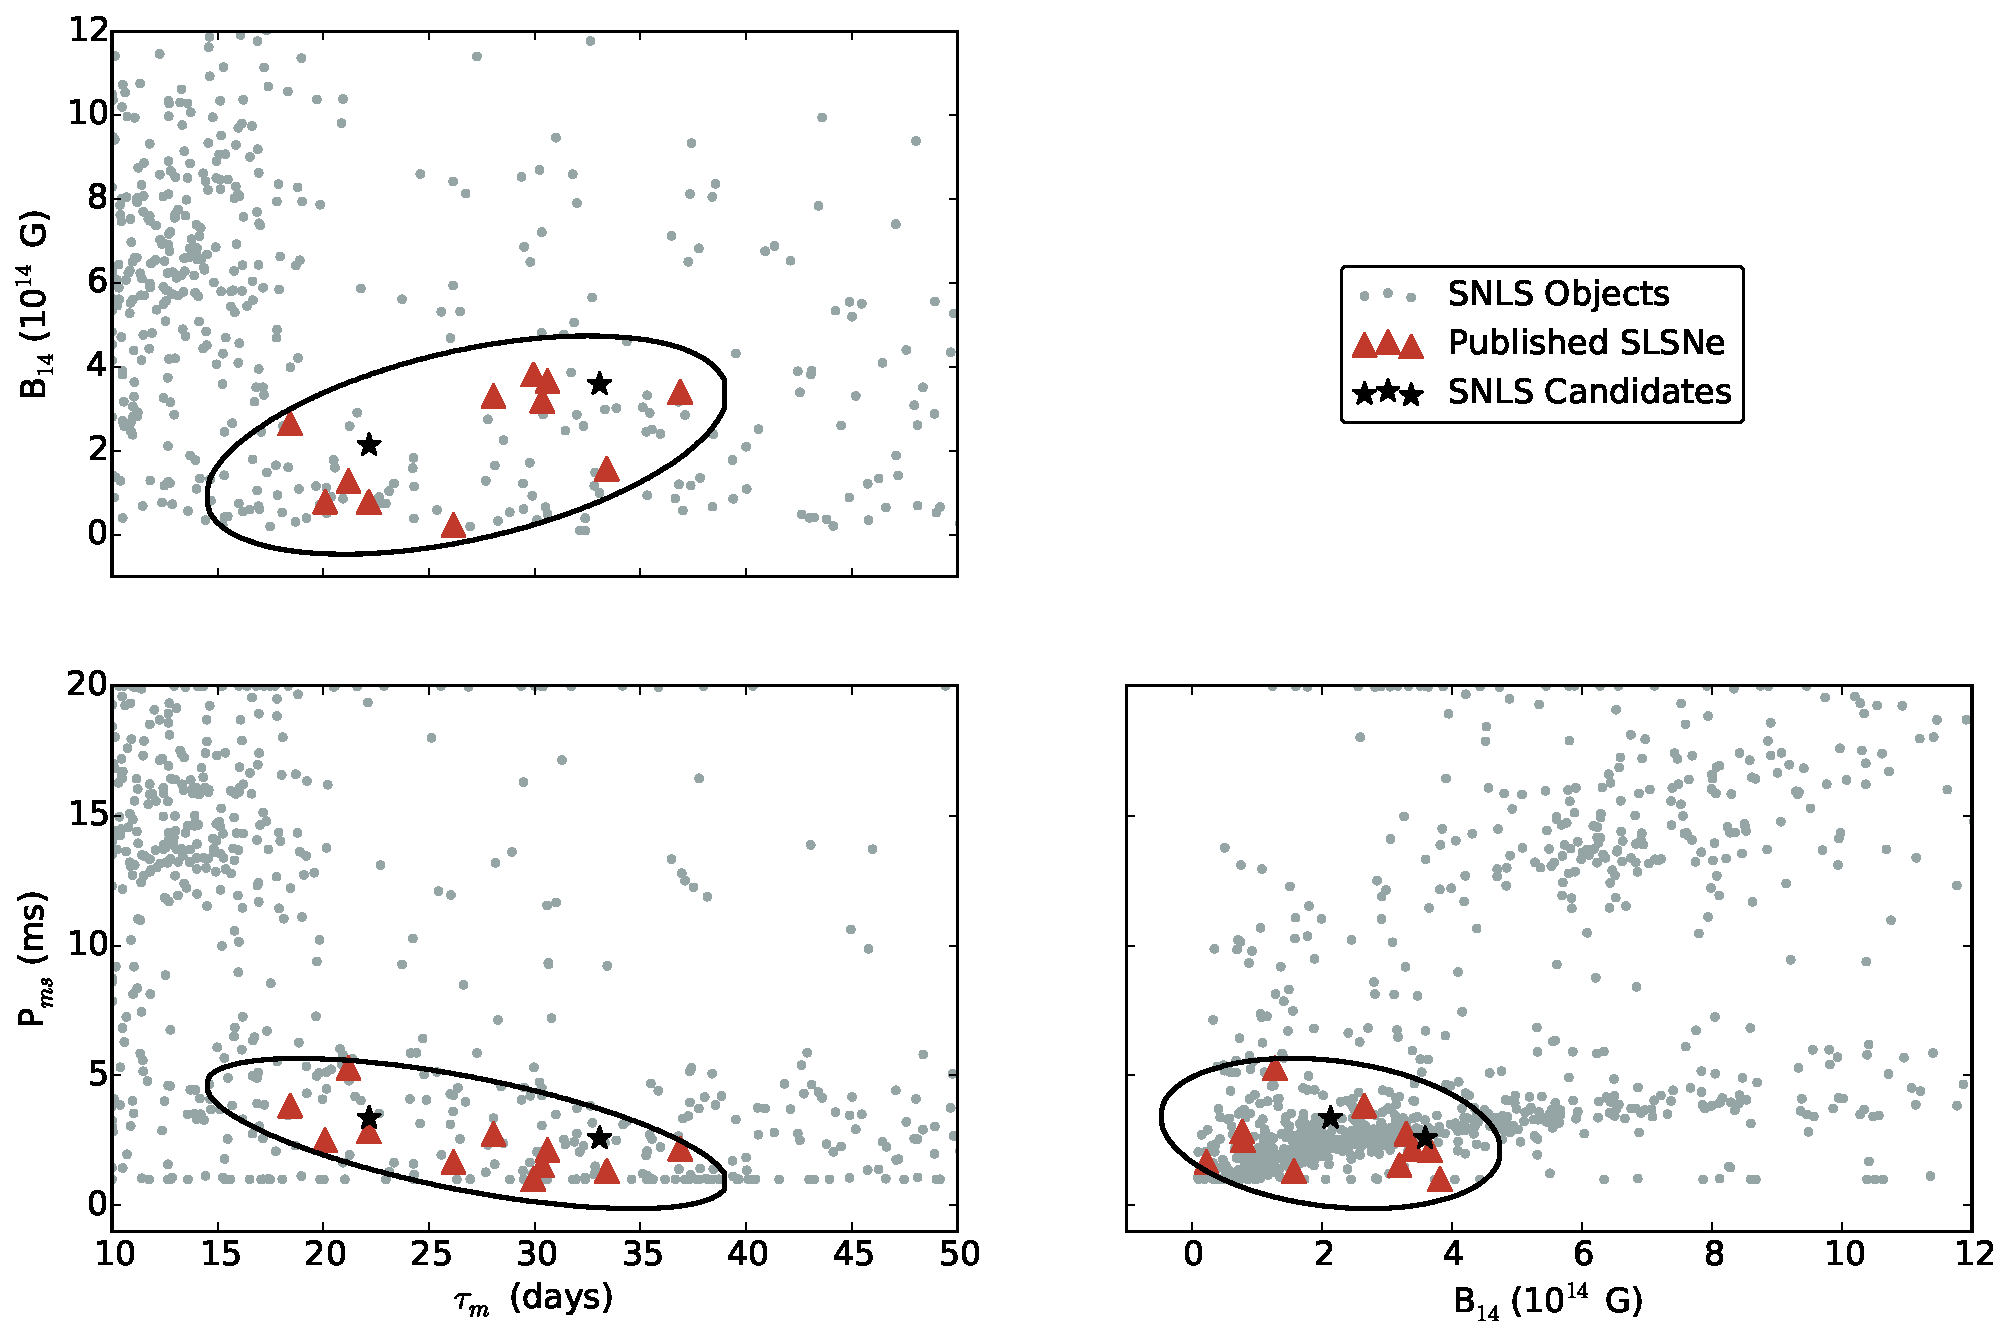
\includegraphics[scale=0.50]{Figures/Chapter3/SLAPparam}
\caption{The $\tau_\mathrm{m}$--$B_{14}$--$P_{\mathrm{ms}}$ parameter space constructed from the magnetar model fits. The SNLS objects are denoted by grey circles. The ellipses correspond to the two dimensional projections of the three dimensional ellipsoid, fitted around the parameter space of the known SLSNe (shown as triangles) to form a region defining them in terms of the model. The SNLS candidates that fall within this parameter space are shown as stars.}
\label{fig:SLAPparam}
\end{figure}

\section{Searching for SLSN in SNLS}
The definition of a SLSN presented in \sref{sec:SLSNDefinition} was then used to classify further objects that were not in our training sample by fitting the magnetar model to those light curves and comparing their best-fits to the parameter space defined by the training sample. In the ideal case we would have first liked to test our definition against a test sample of SLSNe that have not been used in forming of the definition. However, the number of known SLSN events at that time was low enough that we could have not afforded to split it into a training and test samples. We were therefore forced to assume that the parameter space in \fref{fig:SLAPparam} was defined by a representative sample of events. This has further motived us to seek a more elegant and robust solution for any future search of SLSN such as the one performed on the DES dataset in \cref{Chapter5}. I would also like to note that both the fitting method and the definition of a SLSN-like event presented in this chapter does not makes any assumption about the luminosity of the event; making it entirelly possible for fitted events to have $M_u>-21$ and still be classified as SLSNe. Equally, same is true for some events with $M_u<-21$, including those with a relatively short diffusion timescale, $\tau_\mathrm{m}$, giving rise to a faster evolution that is inconsistent with SLSNe. This natural consequence of the technique used here was therefore non susseptable to other classes of luminous (but faster) events \citep{Arcavi15}.

\subsection{Magnetar model fitting}
With the model and definition of SLSNe in place, our next task was to apply the same technique to the sample of SNLS transients. The SNLS detected 4949 transient objects in total \citep{Perrett2010}. This included many objects that were visually designated as active galactic nuclei (AGN) and variable stars, as well as supernovae. In order to perform the fitting on the sample we first has to match each object with a redshift where known. 1694 object in the transient catalogue had spectroscopic redshifts, either from spectra of the transients or of the host galaxy.


As previously described in \sref{sec:SNLSRedshift}, where a spectroscopic redshift is not available, we use photometric redshift estimates. SNLS transients were associated to potential host galaxies by selecting the nearest galaxy within a radius of 1.5''. This provided photometric redshift information on for a further 1527 events. As the photometric redshift estimates are less precise than their spectroscopic counterparts we did not use them directly. Instead, for these transients, we use a range of redshift values spanning the photometric redshift uncertainties. We iterated from the lower to upped uncertainty band in steps of $\Delta$z = 0.04.

At this stage of the analysis we were left with 1728 candidates that had no redshift information. Due to the depth of the SNLS deep stack compare to that of the science images we have expected less objects to be considered 'hostless' as SNLS should have been able to measure photometric redshifts for all but the very faintest host galaxies. We have inspected these objects both visually and using simple statistics. This included the number of detections, number of bands the object was detected in and the separation between detections, and found that a large majority of these objects were in fact likely to be false detections that incidentally matched the SNLS real-time detection criteria \citep{Perrett2010}. Our inspection showed that only 292 of these objects were likely to be real with multiple detections in multiple bands. For these last objects, we have iterated over a broad range of redshifts (0.2 $\leq$ z $\leq$ 1.6 in steps of $\Delta$z = 0.1) but otherwise treated them identically to objects with a known redshift.

Once we have associated every event with a redshift we have proceeded to fitting the SNLS sample using the magnetar model. During the fitting process we have applied the same quality cuts as for our SNLS training sample. We have only accepted objects which had two detections in at least three bands between the best-fit explosion date and maximum light, and a further two detections in at least three filters between maximum light and $+30$ days. For the purpose of this work we considered a detection to be $\geq5$\,$\sigma$ in the real-time photometry. Amongst the 4949 SNLS transients only 2097 had passed our data quality cuts. Their best-fits to the magnetar model are shown in \fref{fig:SLAPparam}.

\subsection{Candidates}
As would be expected, and fortunately for us, the magnetar model was not a good fit to the majority of the SNLS objects. A simple $\chi^2$ test was sufficient to remove a large majority of these poor fits quality objects. We have applied a conservative cut at a $\chi^2$ per degree of freedom ($\chi^2_{\nu}$) of 20. We have chosen such a large $\chi^2_{\nu}$ cut in order to retain all SLSNe including these that might be associated with pre-peak 'bumps' \citep{2015ApJ...807L..18N,2015arXiv151103740N,2016ApJ...818L...8S}. Such objects are well represented by the to the magnetar model in the main part of the event, however, due to the extra undulations, their goodness-of-fit is not ideal when taking into account the whole light curve.

Of the SNLS objects that pass our data quality and $\chi^2_{\nu}$ cuts, four lied within the parameter space of SLSNe as defined in \ref{sec:SLSNDefinition}. This included the two spectroscopically confirmed events from \citet{Howell2013} that were part of our training sample. For the other two candidates, SNLS-05D3ks and SNLS-07D3bs, we measured the multi-season light curves using the custom \textsc{PTFPHOT} pipeline (described in \cref{Chapter2}) to allow us to visually inspect the objects and search for signatures of any long-term variability or detections prior to, or sufficiently after, the putative supernova event. This process of visual inspection has eliminated SNLS-05D3ks which showed clear multiple maxima spanning three years as seen in \fref{fig:05D3ks}. This has left us with just a single, new SLSN-like candidate: SNLS-07D3bs.

\begin{figure}
\centering
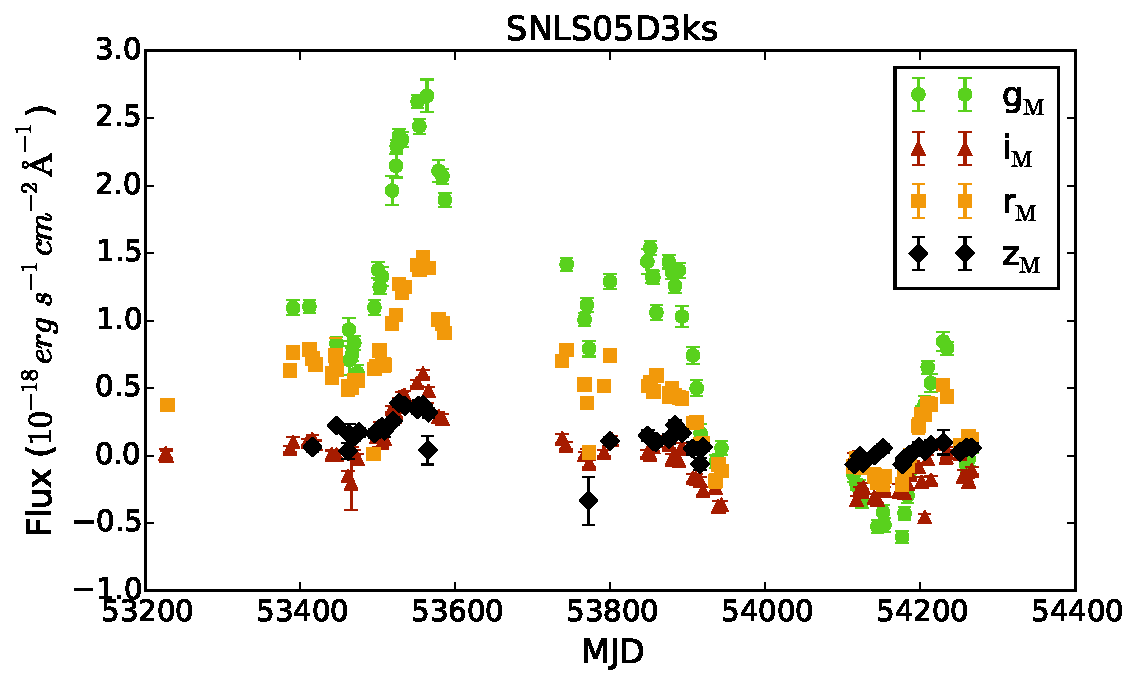
\includegraphics[width=0.5\textwidth]{Figures/Chapter3/SNLS05D3ks}
\caption{The $g_M$, $r_M$, $i_M$, $z_M$ multi-season light curve of SNLS-05D3ks. This transient was found within the SLSN parameter space (\fref{fig:SLAPparam}), but did not pass visual inspection as it showed clear signs of multiple maxima.}
\label{fig:05D3ks}
\end{figure}

\subsection{SNLS-07D3bs}
\label{sec:07D3bs}
SNLS-07D3bs was identified as a SLSN candidate between $0.6<z<1.2$ based on its host galaxy photometric redshift estimate. The best-fit magnetar model for the object was obtained at z=1.0. While SNLS-07D3bs was never classified or recognised as an object of interest during the life of SNLS, it has been spectroscopically observed on the 17$^{\mathrm{th}}$ April 2007 using the Keck/LRIS instrument. This data was never published officially as no spectral classification was obtained at that time. The data was however presented in a PhD thesis by \citet{2013PhDT.......150F}.

At the time the observations of SNLS-07D3bs were made, the SLSN class was not known and no SLSN spectral templates were available for comparison with the data. The SLSN that have been identified in SLSN by \citet{Howell2013} have also been originally not identified as objects of interest until several years after their initial detection. Using the \textsc{superfit} spectrum identification tool \citep{Howell2005}, we have re-analysed the spectrum of SNLS-07D3bs by fitting all available SN templates at a broad range of redshifts exciting our photometric estimate. The data are noisy (signal-to-noise $\sim$ 7) as observing conditions were quite poor. Despite this, we found the best spectral match to be to the SLSN iPTF13ajg at $z=0.757$ as can be seen in \fref{fig:07D3bsSpec}. While this was clearly an uncertain spectral classification, there was no evidence from the spectrum that the object is not a SLSN, particularly as the best match is an event of that type. The magnetar model also provides a good fit at that redshift as seen in  \tref{tab:07d3bsParams}. The host galaxy, located at RA=14h~21m~50.466s, Dec=+53$^{\circ}$~10m~28.58s, was detected in the SNLS deep stack images \citep{Ilbert2006}, but is very faint, with AB magnitudes of ($u_M$, $g_M$, $r_M$, $i_M$, $z_M$) = ($26.61\pm0.49$, $26.13\pm0.16$, $25.67\pm0.13$, $25.18\pm0.11$, $25.19\pm0.37$). Combining the spectral and magnetar model fitting, as well as a faint host galaxy, matching the properties expected of most SLSNe, provided us with sufficient evidence to consider SNLS-07D3bs to be the third SLSN detected by the real-time pipeline of SNLS.

\begin{figure}
\centering
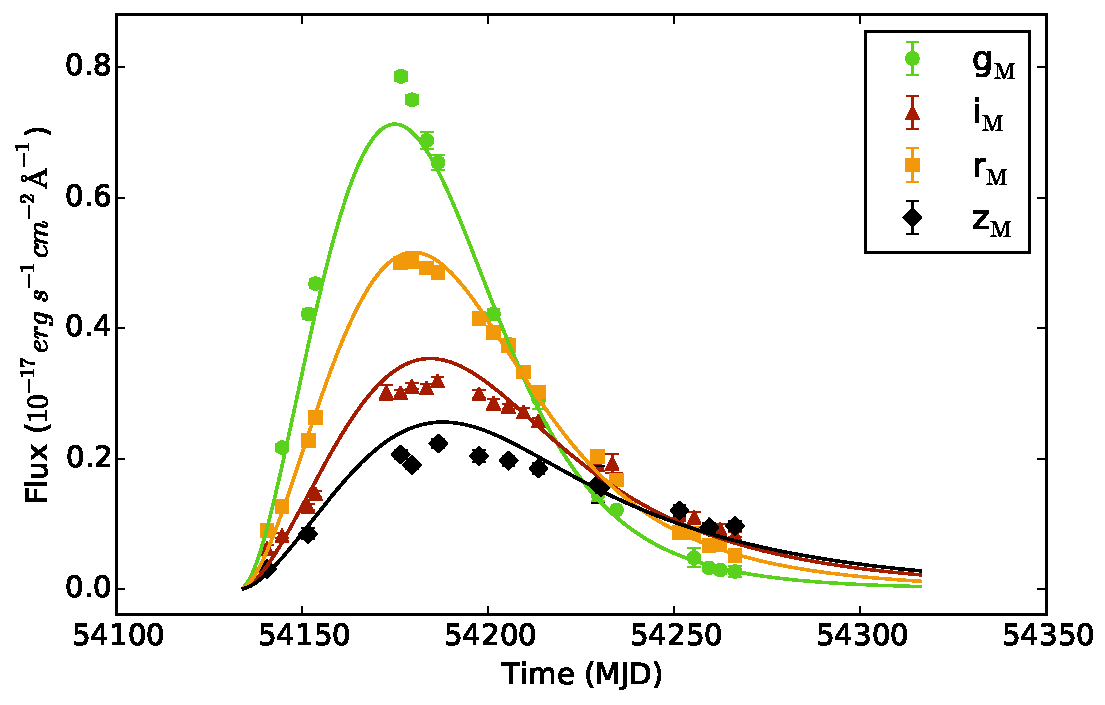
\includegraphics[scale=0.5]{Figures/Chapter3/07D3bs}
\caption{The $g_M$, $r_M$, $i_M$, $z_M$ light curve of SNLS-07D3bs overplotted with the best-fit magnetar model at $z=0.757$. The candidate shows a good agreement with the model.}
\label{fig:07D3bsLC}
\end{figure}

\begin{figure}
\centering
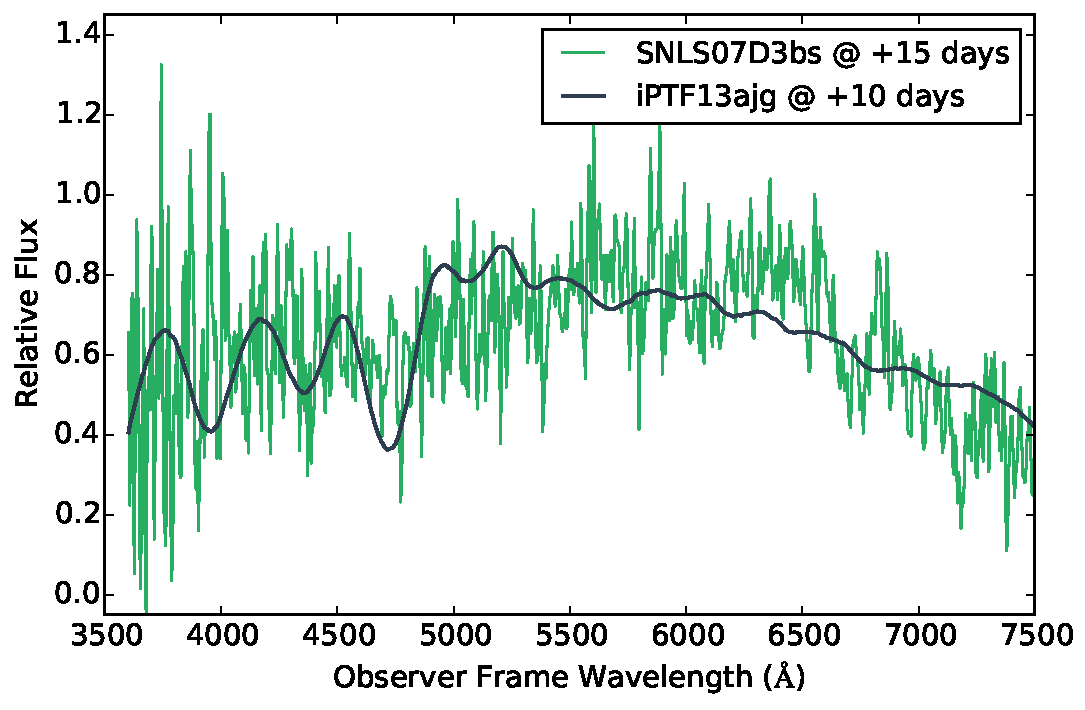
\includegraphics[scale=0.5]{Figures/Chapter3/07D3bsSpec}
\caption{The spectrum of SNLS-07D3bs from Keck/LRIS, taken 15 rest-frame days after maximum light. The signal-to-noise of the spectrum is low preventing a definitive classification; however, the spectrum is consistent with a SLSN at around $z=0.76$. Weak galaxy emission lines are consistent with $z=0.757$.}
\label{fig:07D3bsSpec}
\end{figure}

\begin{table}
\begin{center}
\caption{Magnetar model parameters for the new SNLS SLSN candidate: SNLS-07D3bs.}
\label{tab:07d3bsParams}
\begin{tabular}{|l|r|r|r|r|r|r|r|r|r|r|}
\hline
  \multicolumn{1}{|c|}{Name} &
  \multicolumn{1}{c|}{$M_u$} &
  \multicolumn{1}{c|}{$t_\mathrm{rise}$} &
  \multicolumn{1}{c|}{$\tau_\mathrm{m}$} &
  \multicolumn{1}{c|}{$B_{14}$} &
  \multicolumn{1}{c|}{$P_{\mathrm{ms}}$} &
  \multicolumn{1}{c|}{$t_\mathrm{expl}$} &
  \multicolumn{1}{c|}{$E(B-V)$} &
  \multicolumn{1}{c|}{$\chi^2_{\nu}$} &
  \multicolumn{1}{c|}{Template} \\ & &
  \multicolumn{1}{c|}{(days)} &
  \multicolumn{1}{c|}{(days)} &
  \multicolumn{1}{c|}{($\times10^{14}$ G)} &
  \multicolumn{1}{c|}{(ms)} &
  \multicolumn{1}{c|}{(MJD)} & \\
\hline
SNLS-07D3bs & -20.9 &  27.2 & 23.7 & 2.28 & 3.81 & 54132.5 & 0.05 & 1.96 & iPTF13ajg\\
\hline
\end{tabular}
\end{center}
\end{table}
